% 4_5_SchoolIntervention.tex

\subsection{School Intervention}
This section evaluates the impact of targeted social distancing by simulating a school closure scenario across the four network models.
Rather than physically removing edges, the intervention is modeled as a probabilistic reduction by manipulating the underlying generative parameters.

\subsubsection{Definition and Target of Intervention}
In the structured Model 2B, the school intervention is defined by neutralizing the coefficients associated with educational settings.
Specifically, we modify Equation \ref{eq:m2b_full} by setting the parameters for school cohorts to zero: $\gamma_{pri\_low} = \gamma_{pri\_high} = \gamma_{sec} = \gamma_{ter} = 0$.
This allows us to calculate the intervention-adjusted contact probability, $P_{ij}^{close}$, for all pairs meeting the age-mixing criteria defined in Section \ref{sec:network_model}.
The baseline probabilities, $P_{ij}^{open}$, represent the state where schools are fully operational.

\subsubsection{Quantification of Reduction Factor}
To ensure a consistent magnitude of intervention across all models, we derived a standardized reduction factor, $R_{val}$.
This factor is calculated as the ratio of the total expected edges in the intervention scenario to those in the baseline scenario for the school-eligible population.
Let $\Omega$ be the set of individual pairs $(i, j)$ that satisfy the school cohort criteria.
The reduction factor is defined as:
\begin{equation}
    R_{val} = \frac{\sum_{(i,j) \in \Omega} P_{ij}^{close}}{\sum_{(i,j) \in \Omega} P_{ij}^{open}}.
\end{equation}
Based on our Model 2B posterior estimates, the calculated $R_{val}$ was approximately $0.2218$.
This indicates that a complete school closure corresponds to a reduction of approximately 77.8\% in the probability of contact between eligible youths within educational settings.

\subsubsection{Application to Baseline Models}
The reduction factor $R_{val}$ is subsequently applied to the Erd\H{o}s-R\'enyi and Model 1 networks to facilitate a fair comparison.
We identify "eligible" pairs in these models that satisfy the same age and age-difference boundaries as the school cohorts in Model 2B.
For these identified pairs, the baseline contact probability $P_{ij}^{M1, base}$ is scaled by the reduction factor:
\begin{equation}
    P_{ij}^{M1, interv} = P_{ij}^{M1, base} \times R_{val}.
\end{equation}
This methodology ensures that the total volume of contact reduction is identical across all models.
For the Erd\H{o}s-R\'enyi network, this reduction is operationalized by stochastically pruning edges of eligible pairs with probability $R_{val}$.
Crucially, during the subsequent SIR simulations, the per-contact transmission probability $\rho$ was kept constant at the baseline value.
This ensures that the pathogen's intrinsic infectiousness remains unaffected, allowing us to isolate the topological impact of the intervention.

\subsubsection{Comparative Analysis of Simulation Results}
Stochastic SIR simulations were performed to analyze the effectiveness of the intervention across different topologies, as visualized in Figure \ref{fig:sir_comparison}.
The results demonstrate that the effectiveness of school closure is highly sensitive to the underlying network structure.
In the Erd\H{o}s-R\'enyi model, the intervention yielded negligible changes in the epidemic trajectory, as the pathogen easily bypassed the localized reductions through the homogeneous background of contacts.
In Model 1, the average infection peak decreased from 2,634 to 2,545 individuals, representing a marginal reduction of only 3.37\%.
In contrast, Model 2B exhibited a significant suppression of the outbreak, with the peak incidence dropping from 2,604 to 2,282 individuals.
This substantial 12.3\% reduction in Model 2B is particularly noteworthy because it was achieved with the exact same volume of contact reduction as in Model 1.
The discrepancy highlights that in structured networks, school cohorts act as dense "transmission engines" or hubs.
Neutralizing these specific structural clusters breaks the core connectivity of the virus, leading to a non-linear suppression of the global peak.

\begin{figure}[H]
    \centering
    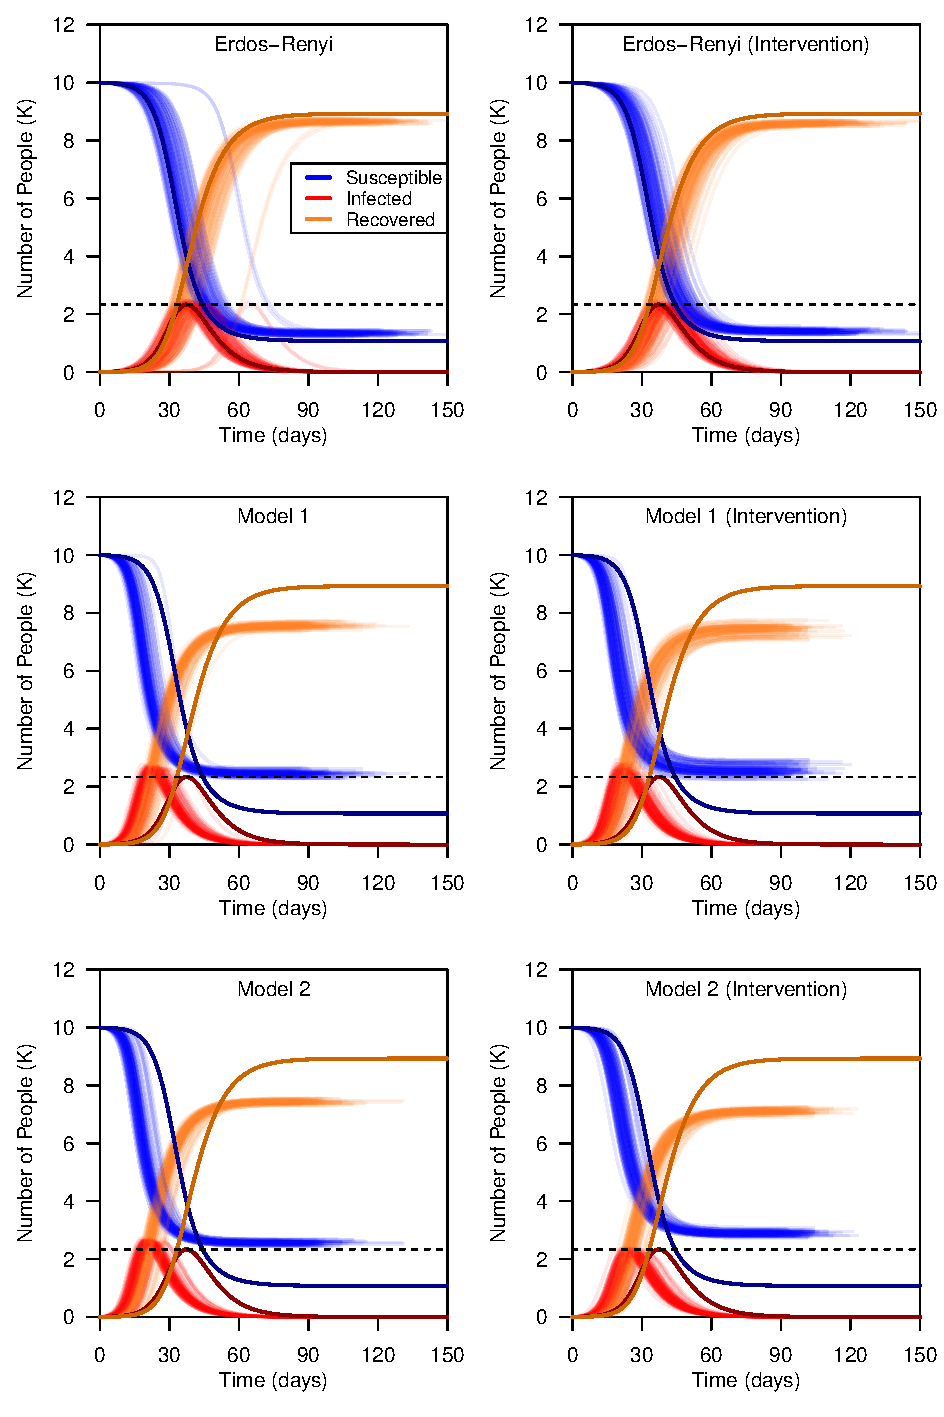
\includegraphics[width=0.8\linewidth]{figures/04_EpidemicModel/sir_comparison_r0_25.pdf}
    \caption{Comparison of SIR trajectories between Baseline and School Intervention scenarios ($R_0=2.5$). While the intervention has minimal impact on homogeneous models, it significantly suppresses the infection peak in Model 2B by dismantling dense school clusters.}
    \label{fig:sir_comparison}
\end{figure}

\subsubsection{Policy Implications and Limitations}
The findings of this study provide two critical insights for public health policy: the risk of overlooking epidemic acceleration and the potential for highly effective, targeted interventions.
First, the integration of realistic social layers reveals a significant risk of epidemic acceleration that is systematically overlooked in homogeneous models.
Our results demonstrate that when an outbreak occurs within structured environments like school cohorts, the pathogen exploits a high-speed "transmission highway" facilitated by dense local connectivity and high assortativity.
In these scenarios, the infection peak occurs both higher and significantly earlier than predicted by Mean Field or Erd\H{o}s-R\'enyi models.
Relying on oversimplified models for forecasting thus creates a dangerous "blind spot," where policymakers may systematically underestimate the urgency required for early-stage interventions.
Our model suggests that the window for effective peak suppression is much narrower than traditional models imply, making the timing of intervention as critical as its magnitude.

Second, the structural analysis identifies specific societal layers where interventions can yield disproportionately large impacts.
The 12.3\% reduction in the infection peak observed in Model 2B compared to only 3.37\% in Model 1 for the same volume of contact reduction proves that neutralizing "transmission engines" such as schools can non-linearly suppress the global outbreak.
This highlights the necessity of structured modeling to identify critical nodes and layers for precision public health strategies.

However, it is important to acknowledge that the potent suppression observed in Model 2B represents an optimistic scenario.
The model assumes that the edges removed through school closure are not replaced by other forms of interaction.
In reality, school closures may trigger "contact substitution," where students replace institutional interactions with informal social activities in the community.
Empirical evidence suggests that such behavioral shifts can significantly increase contacts within households and other private settings, potentially diminishing the intended impact of the closure \parencite{litvinova2019reactive}.
Such behavioral shifts could re-introduce random connectivity, potentially causing the network to revert toward a Model 1-like structure and diminishing the overall effectiveness of the policy.
Future research should incorporate these behavioral feedback loops to refine the predictability of layer-specific interventions and account for the dynamic nature of human sociality during a crisis.